\chapter{LaTeX 方案与总结}
\label{chap:3}

\subsection{LaTeX 方案}

由于该作业最后需要使用 LaTeX 进行呈现,在此本作业选择使用 Overleaf 进行开发工具的选项,同时本作业也考虑到之后在不同作业与不同状况下有可能遇到的问题,所以特别进行不同的方案,为之后有可能遇到的状况进行准备。

LaTeX 为一种基于 TeX 而开发的文件排版系统,其优势在于进行编排档时可以进行版控,同时该方案所产生的 PDF 档内容极小,但劣势则是在于在一些情况下,撰写的时间会比较费力,若要符合一般的档需求,则使用目前的文书编辑软件与工具,甚至是商用的在线文书编辑平台来进行工作。当然也有开源跨平台授权的文书软件方案。

在此考虑下,本地端可以考虑使用 Texmaker ,其优势原因在于开源,该软件是专门支持 LaTeX 的图形接口功能,只要事先装好 MiKTeX 等 LaTeX 的开发环境,就可以快速投入工作流程。而 Overleaf 则是商业的多人跨平台协作方案,其最佳的优势在于支持多人协作与版本控制,而且初学者不用考虑到 LaTeX 在本地端较复杂的环境维护,另外 Overleaf 还有许多志愿者所贡献的模板,而本作业就是使用 Overleaf 平台上名为  iofu728 所提供的北京大学硕士论文格式模板。最后回到两者的方案上,前者 Texmaker 可以提供直觉化的图形接口操作,不受网络环境影响的本地端 LaTeX 开发环境,同时后者的 Overleaf 则是在快速开发、多人协作与容易入门上,占有极大的竞争优势,两者相辅相成。

最后整理出使用者在面对 LaTeX 学习门坎最高的数学式跟符号问题,在此有三种可以辅助的方式,其一为 Mathpix Snip 的 OCR 辨识转 LaTeX 的数学式符号输出,该方案需要注册平台后,其使用者就可以使用指定的版本,此外在 Texmaker 当中就有特定符号的图形化接口操作,而目前 MS Office 2019 版本在数学式上也有支持 LaTeX 的转换,虽然在一些细节上处理并没有很好,但是已经可以面对大量的工作量需求。


\begin{figure}[htb]
\centering 
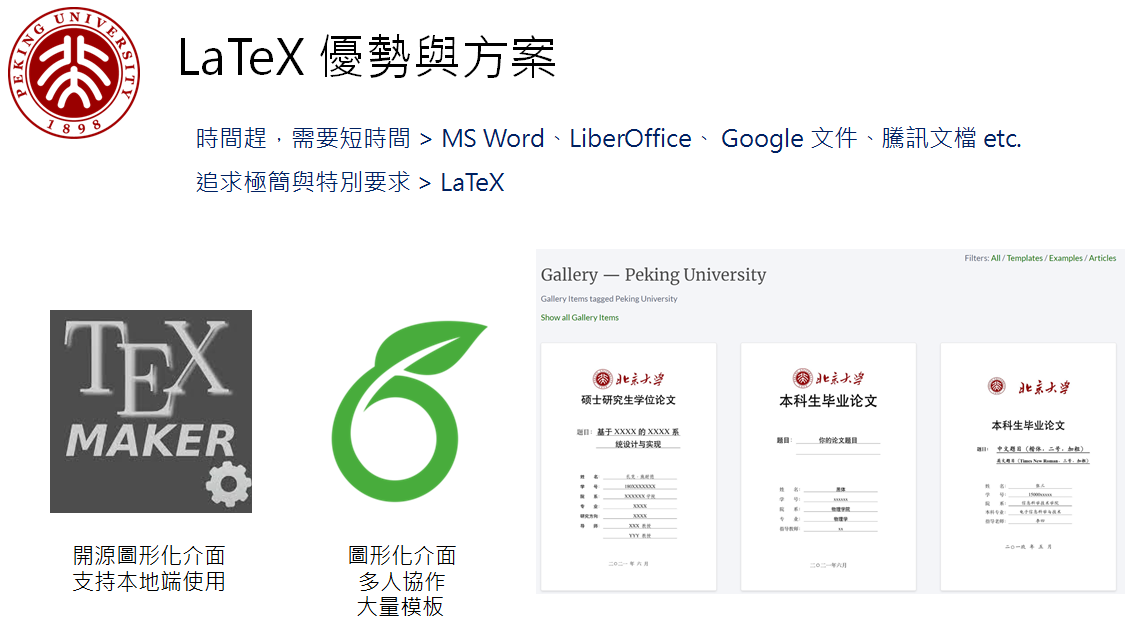
\includegraphics[width=0.90\textwidth]{img/c3m0.png} 
\caption{LaTeX 的方案}
\label{Test}
\end{figure}

\begin{figure}[htb]
\centering 
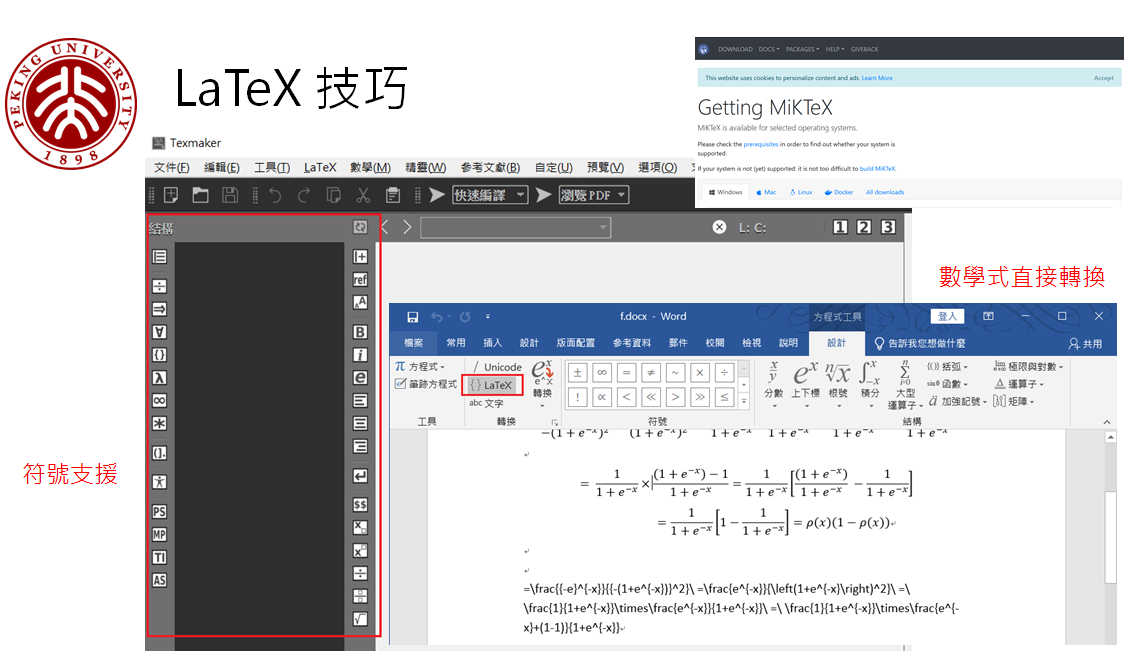
\includegraphics[width=0.90\textwidth]{img/c3m1.png} 
\caption{LaTeX 的快速加工}
\label{Test}
\end{figure}

\begin{figure}[htb]
\centering 
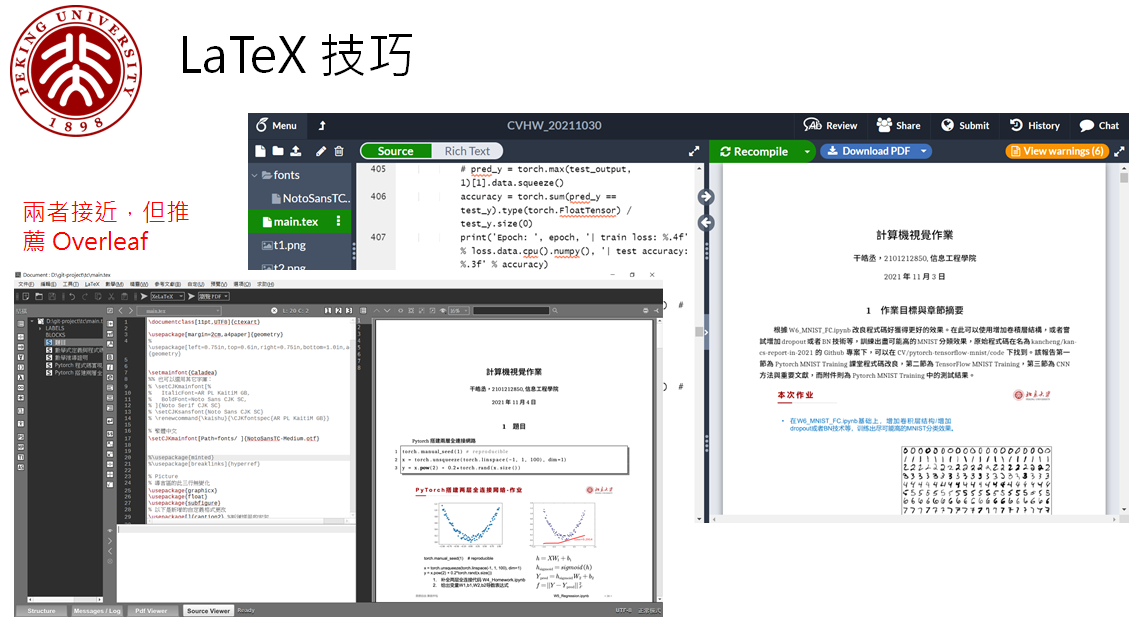
\includegraphics[width=0.90\textwidth]{img/c3m2.png} 
\caption{LaTeX 方案比較}
\label{Test}
\end{figure}

\begin{figure}[htb]
\centering 
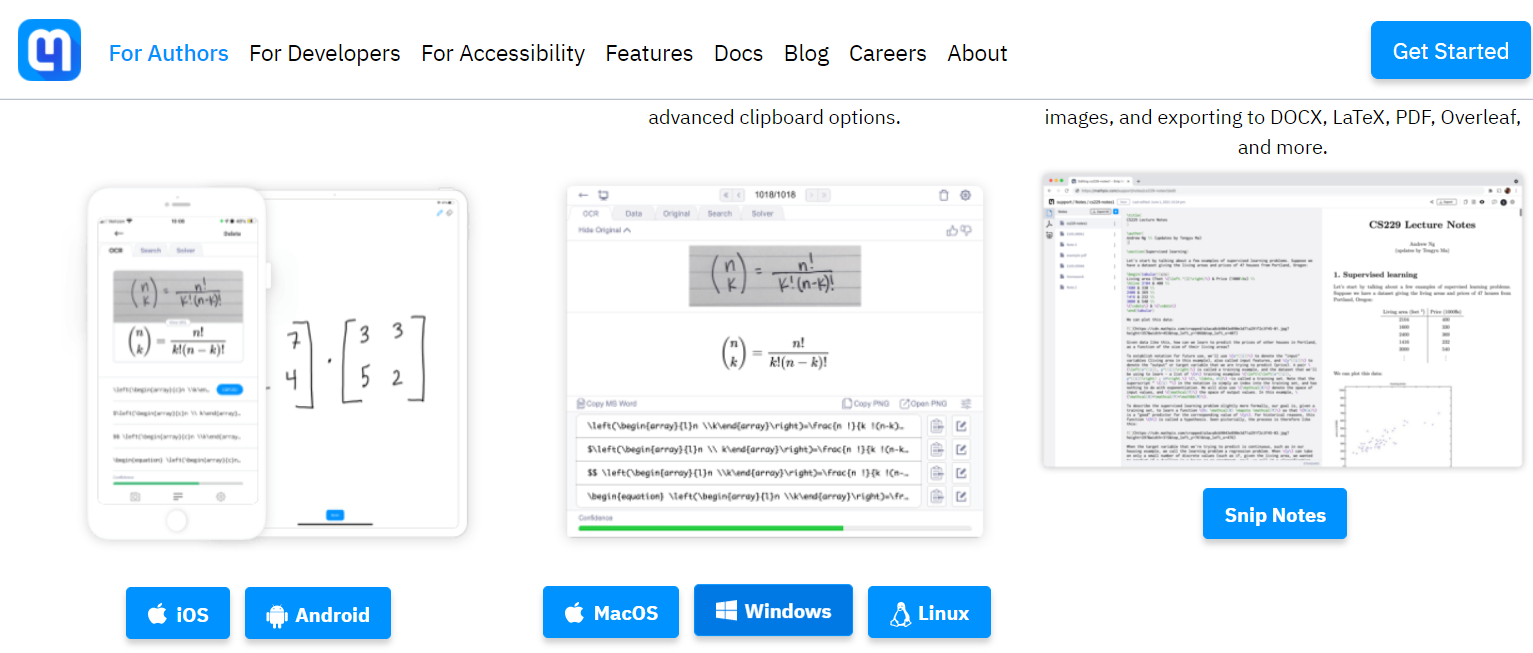
\includegraphics[width=0.90\textwidth]{img/c3m3.png} 
\caption{Mathpix Snip 的 LaTeX 方案}
\label{Test}
\end{figure}

\begin{figure}[htb]
\centering 
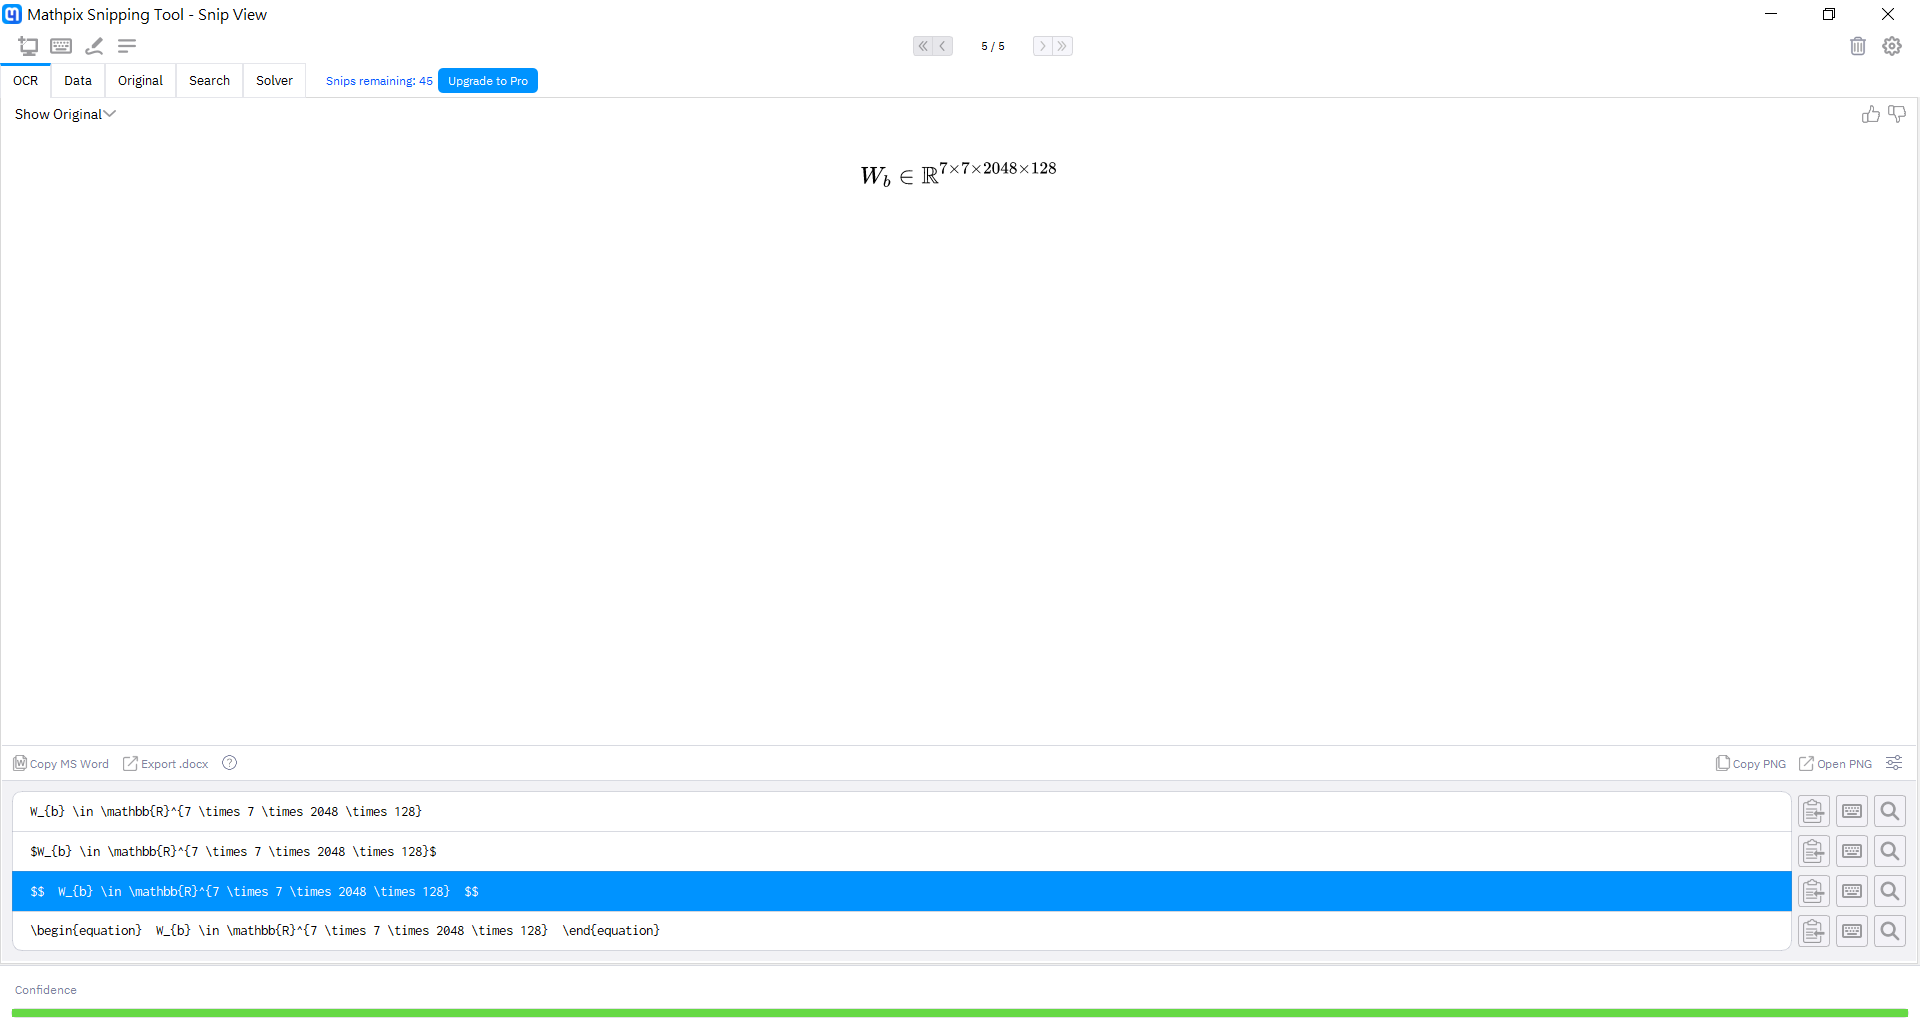
\includegraphics[width=0.90\textwidth]{img/c3m4.png} 
\caption{LaTeX - Mathpix Snip 數學式 OCR 輸出}
\label{Test}
\end{figure}

\subsection{总结}

此作业经过论文精读与全文翻译,同时也研究在 LaTeX 在不同环境下的两种应对方案,前者为 Texmaker 面对本地端稳定的直觉式开发环境,而后者 Overleaf 择重点在快速开发、降低门槛还有多人协作上的优点,并在过程中接触偏大规模的 LaTeX 撰写与研究,并在过程中了解 LaTeX 实际底层的运作跟环境维护,另外也研究了文献管理软体的操作跟时下主要的文献管理软体的优缺点。最后在搜集文献的过程中获得面对研究方向文献收集的经验。